\documentclass{article}

\usepackage{tikz} 
\usetikzlibrary{automata, positioning, arrows} 

\usepackage{amsthm}
\usepackage{amsfonts}
\usepackage{amsmath}
\usepackage{amssymb}
\usepackage{fullpage}
\usepackage{color}
\usepackage{parskip}
\usepackage{graphicx}
\usepackage{hyperref}
  \hypersetup{
    colorlinks = true,
    urlcolor = blue,       % color of external links using \href
    linkcolor= blue,       % color of internal links 
    citecolor= blue,       % color of links to bibliography
    filecolor= blue,        % color of file links
    }
    
\usepackage{listings}
\usepackage[utf8]{inputenc}                                                    
\usepackage[T1]{fontenc}                                                       

\definecolor{dkgreen}{rgb}{0,0.6,0}
\definecolor{gray}{rgb}{0.5,0.5,0.5}
\definecolor{mauve}{rgb}{0.58,0,0.82}

\lstset{frame=tb,
  language=haskell,
  aboveskip=3mm,
  belowskip=3mm,
  showstringspaces=false,
  columns=flexible,
  basicstyle={\small\ttfamily},
  numbers=none,
  numberstyle=\tiny\color{gray},
  keywordstyle=\color{blue},
  commentstyle=\color{dkgreen},
  stringstyle=\color{mauve},
  breaklines=true,
  breakatwhitespace=true,
  tabsize=3
}

\newtheoremstyle{theorem}
  {\topsep}   % ABOVESPACE
  {\topsep}   % BELOWSPACE
  {\itshape\/}  % BODYFONT
  {0pt}       % INDENT (empty value is the same as 0pt)
  {\bfseries} % HEADFONT
  {.}         % HEADPUNCT
  {5pt plus 1pt minus 1pt} % HEADSPACE
  {}          % CUSTOM-HEAD-SPEC
\theoremstyle{theorem} 
   \newtheorem{theorem}{Theorem}[section]
   \newtheorem{corollary}[theorem]{Corollary}
   \newtheorem{lemma}[theorem]{Lemma}
   \newtheorem{proposition}[theorem]{Proposition}
\theoremstyle{definition}
   \newtheorem{definition}[theorem]{Definition}
   \newtheorem{example}[theorem]{Example}
\theoremstyle{remark}    
  \newtheorem{remark}[theorem]{Remark}

\title{CPSC-354 Report}
\author{Brandon Foley \\ Chapman University}

\date{\today} 

\begin{document}

\maketitle

\begin{abstract}
\end{abstract}

\setcounter{tocdepth}{3}
\tableofcontents

\section{Introduction}\label{intro}

\section{Week by Week}\label{homework}

\subsection{Week 1}

\subsubsection{Homework}

Here is my work on the MU Puzzle:

\[
MIU \to MIUIU \to MIUIUIU \to \cdots
\]

\[
MI \to MII \to MIIII \to MUI \quad \Rightarrow \quad MUI
\]

\[
MUI \to MUIU
\]

\[
MUI \to MUIU \to MUIUIU \to MUIUIUIU \to MUUIU \to MUUIUIU \to \cdots
\]

\[
MUIIU \to MUIIUUIU \to MUIU
\]

\[
MUIIU \to MUUIU \to MUIU
\]

\[
MUIU \to MUUIU \to MUIUIU \to MUIUIUIU \to \cdots
\]

\[
MUIUIUIU \to MUIUIUIUIU \to MUIUIUIUIUIU \to \cdots
\]


The MU Puzzle is unsolvable because it is impossible to reach the string \texttt{MU} starting from \texttt{MI} using the given rules.  
After a little research and thinking on my part it is the number of \texttt{I}'s that make this impossible: 
rule applications can double the count, add one, or remove three at a time,  
however, none of these operations ever reduce the number of \texttt{I}'s to exactly zero.  
Since \texttt{MU} has no \texttt{I}'s, it can never be derived.  

\subsubsection{Questions}

What rules could we add or remove in order to make this possible? I was thinking are there any ways to make this question solvable
by adding only one more rule or maybe altering a rule. I think that this is an interesting question and concept.

\subsection{Week 2}

\subsubsection{Homework}

Here is my work on the Rewriting Homework:

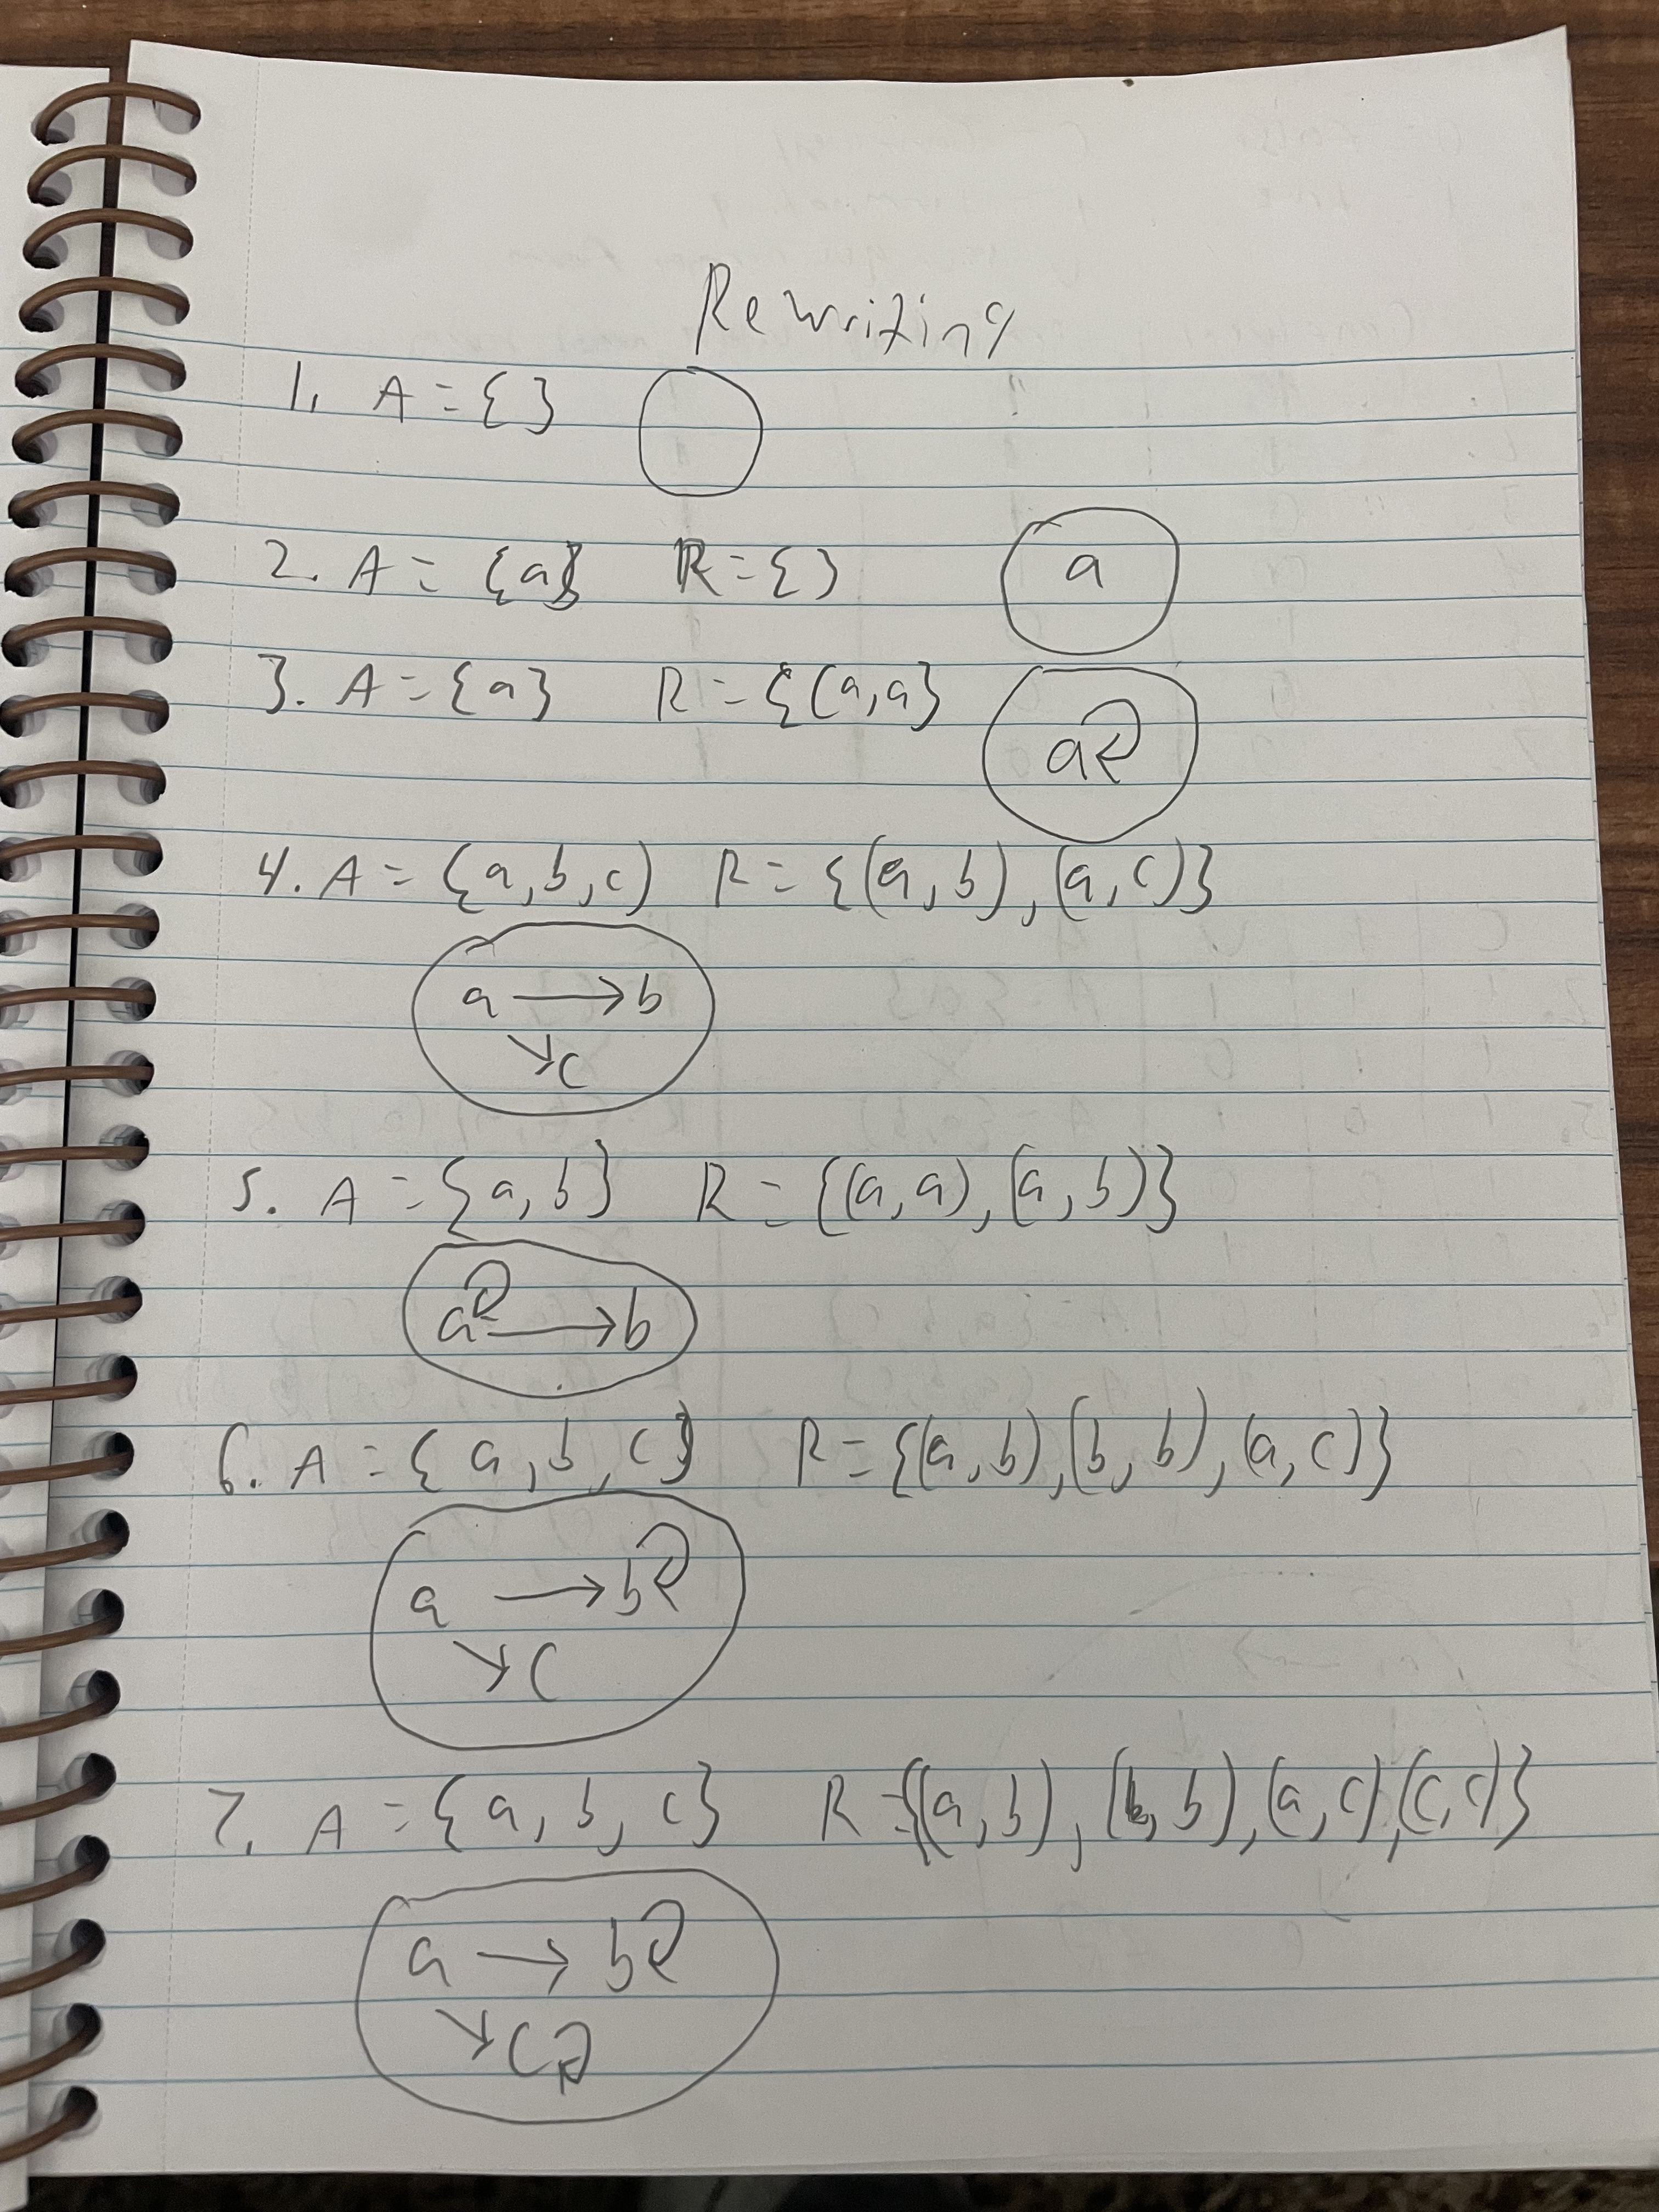
\includegraphics[width=0.8\textwidth]{../img/IMG_2709.jpg}

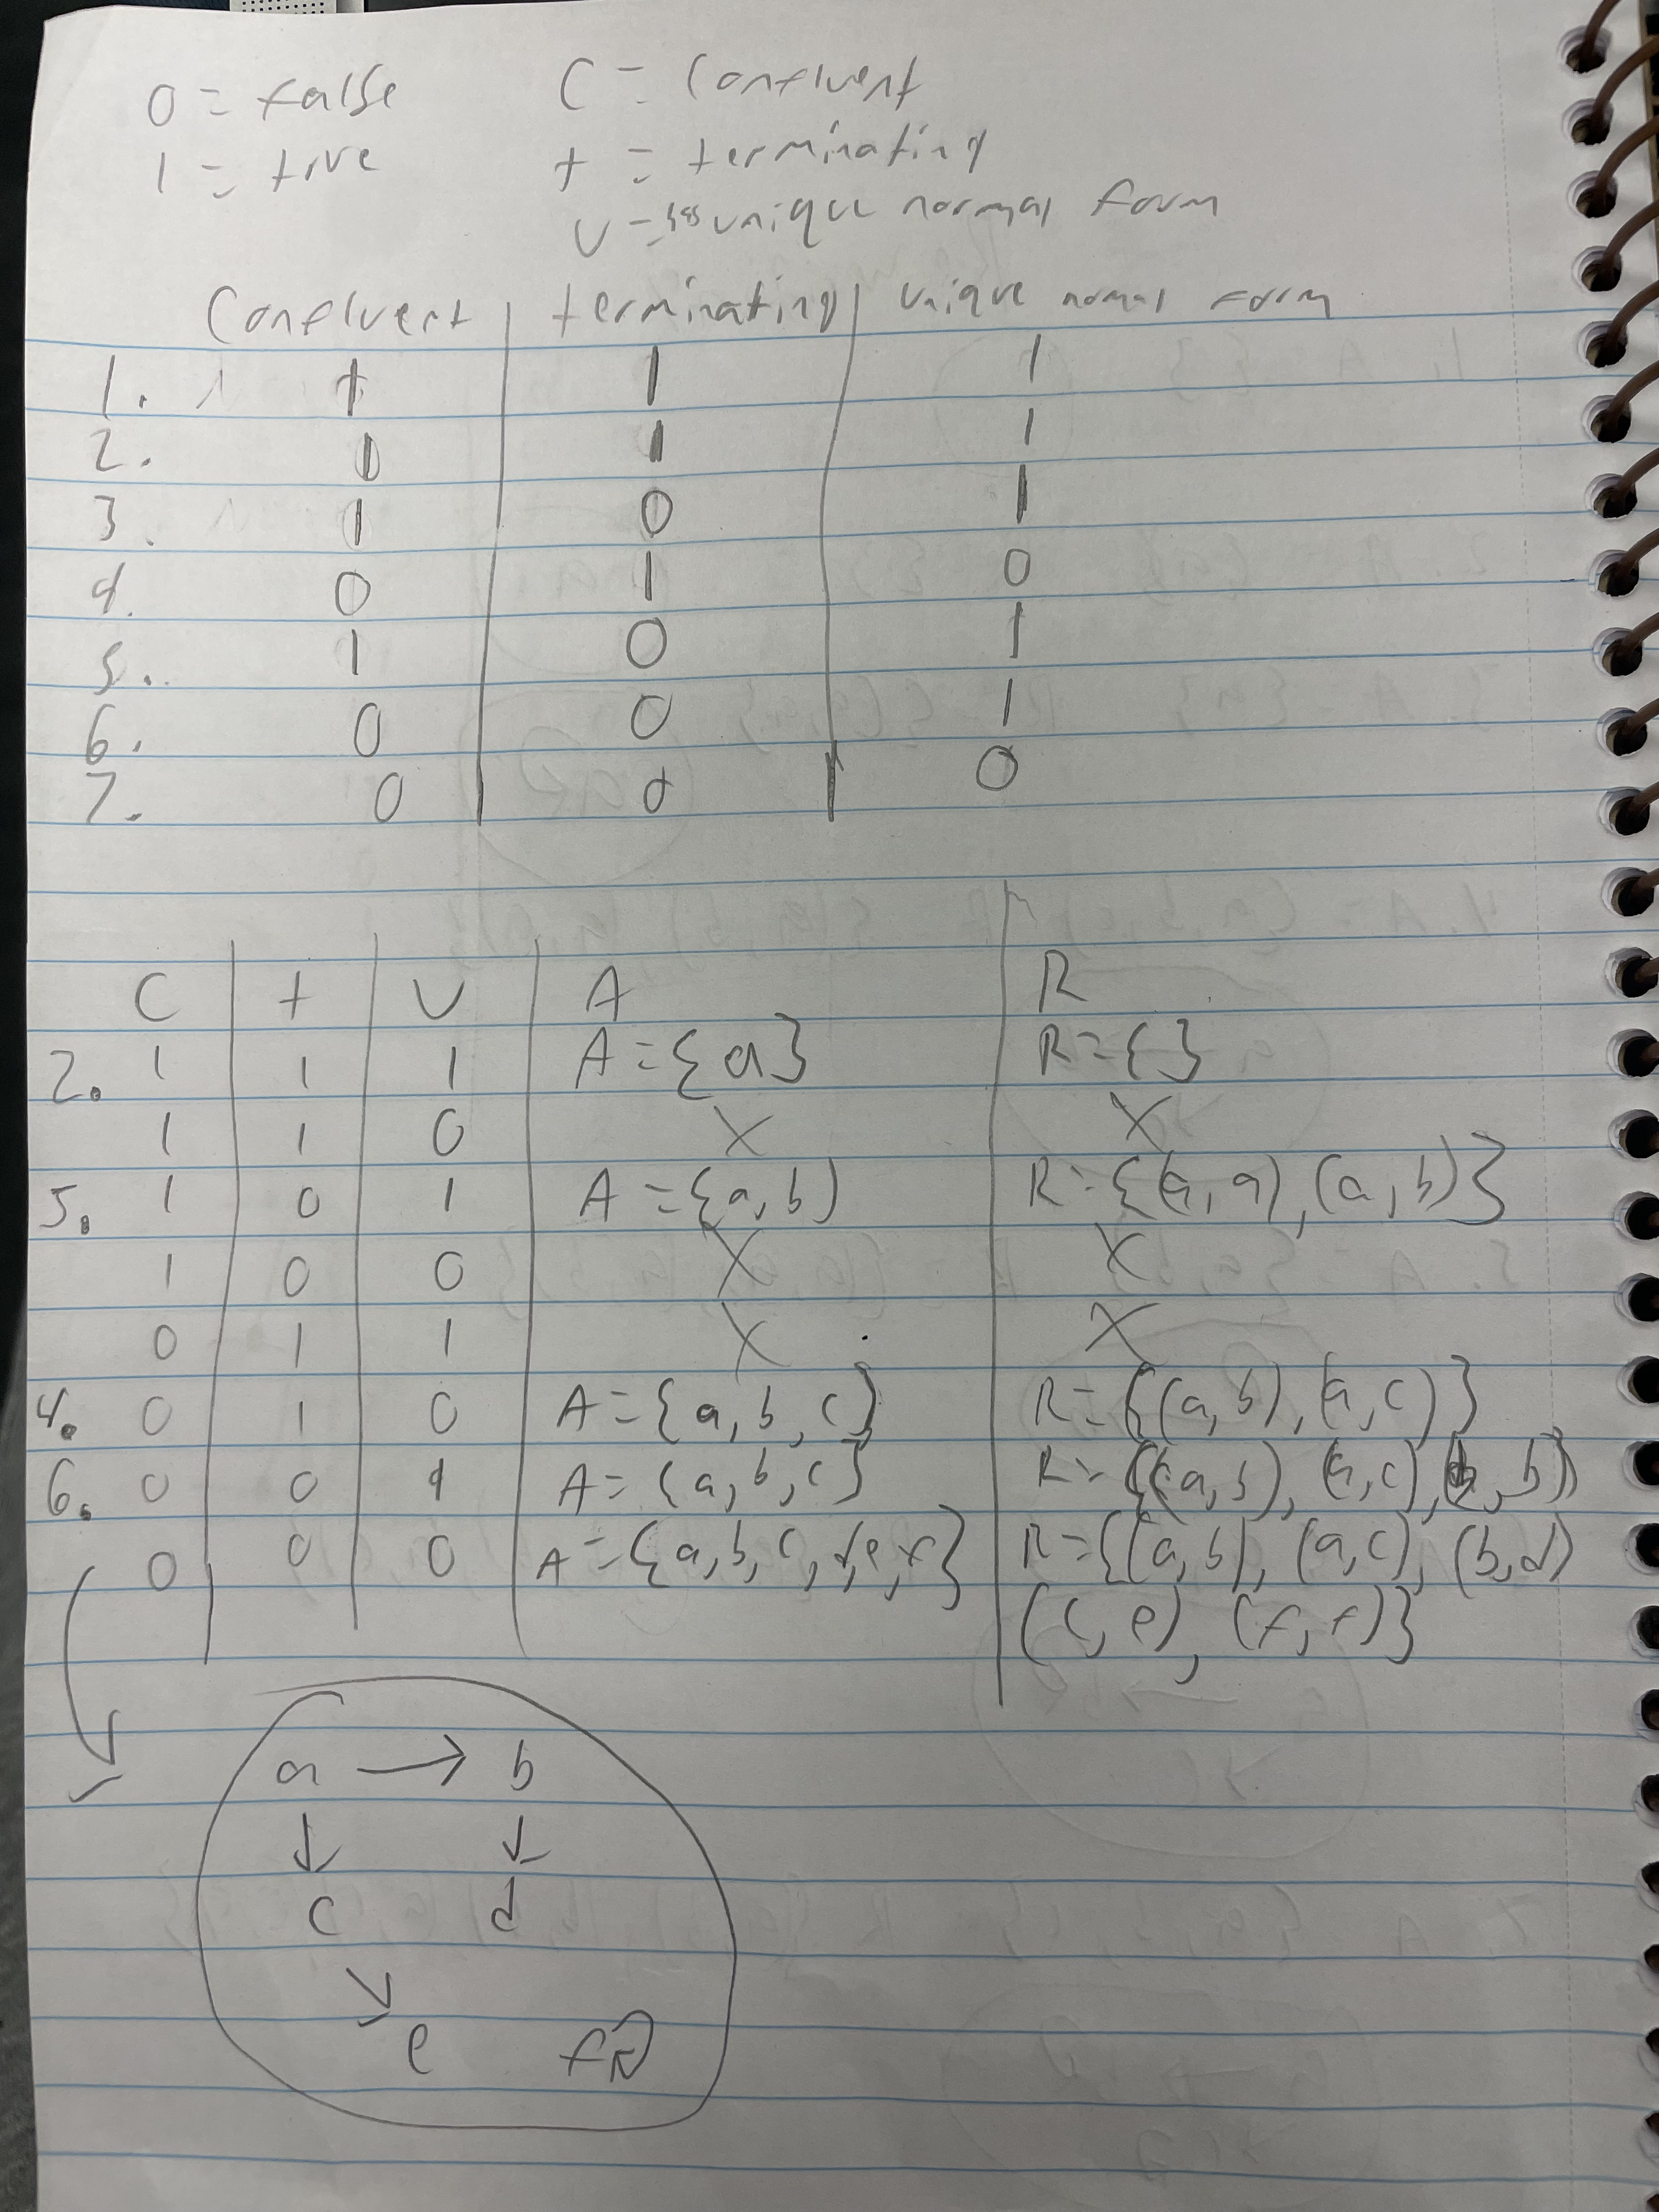
\includegraphics[width=0.8\textwidth]{../img/IMG_2710.jpg}

\subsubsection{Questions}

When relating to programming, if a system is confluent but not terminating, like in some programs with infinite loops, how does confluence still guarantee that the result of a program is unique when it exists?

\section{Essay}

\section{Evidence of Participation}

\section{Conclusion}\label{conclusion}

\begin{thebibliography}{99}
\bibitem[BLA]{bla} Author, \href{https://en.wikipedia.org/wiki/LaTeX}{Title}, Publisher, Year.
\end{thebibliography}

\end{document}
